\documentclass[12pt]{article}
\usepackage{tikz}
\usepackage{blindtext}
\usepackage{multicol}
\setlength{\columnsep}{1cm}
\title{Second multicols Demo}
\usetikzlibrary{calc}
\usepackage{graphicx}
\graphicspath{{images/}}
\usepackage[left=25mm,right=25mm,top=25mm,bottom=25mm,paper=a4paper]{geometry}
\usepackage{graphicx}
\graphicspath{{images/}}

\begin{document}

 \begin{center}
 \large \textbf {A Report on}\\[2mm]
 \LARGE \textbf {"Pc Remote Controller"}\\[7mm]
 
 \textbf{Submitted by :}\\[2mm]
 \end{center}
 
 
 \begin{tabular}{ c c c } 
 \textbf{Mr.Atharv Miind Davale} & \hspace{1in} & \textbf{ PRN :  2020032500183191} \\ [1mm] 
 \textbf {Mr.Rushikesh Rajesh Waghule} & \hspace{1in} & \textbf{PRN :2020032500186525}\\[1mm]
 \textbf{ Mr.Digvijay Sambhaji Shinde } & \hspace{1in}  & \textbf{PRN : :2020032500185166}\\[1mm]
\textbf{ Mr.Abhijeet Balkrishna Surshetwar} & \hspace{1in}  & \textbf{PRN : :2020032500183392}\\[1mm]
\textbf{ Mr.Amrut Yoesh Virdhe} & \hspace{1in}  & \textbf{PRN : :2020032500185916}\\[7mm] 
\end{tabular} 
 
 
 
 \begin{center}
 \large \textbf {UNDER THE GUIDANCE OF }\\[2mm]
 \large \textbf {Mr.A.M.Dyade}\\[7mm]
 \textbf {in partial fulfilment for the award of the degree} \\[2mm] of \\[2mm]
 
 \large \textbf {BACHELOR OF TECHNOLOGY}\\[2mm]
 \textbf {IN}\\[2mm]
 \textbf {DEPARTMENT OF COMPUTER SCIENCE AND ENGINEERING}\\
 \textbf {at}
 \end{center}
 
 \begin{figure}[h]
 \centering
 \includegraphics[scale=1]{sveri2logo}
\end{figure} 

\begin{center}
\textbf{SHRI VITHAL EDUCATION AND RESEARCH INSTITUTESs,\\[2mm]
College of Engineering, Pandharpur\\[3mm]
Affiliated to Punyashlok Ahilyadevi Holkar Solapur University, Solapur\\[2mm]
2023-2024}
\end{center}  
 
 \begin{tikzpicture}
[remember picture,overlay]\draw[line width = 1pt]($(current page.north west)+(0.5 in,-0.5in)$) rectangle ($(current page.south east)+(-0.5 in,1 in)$);
\end{tikzpicture} 
\clearpage


\begin{figure}[h]
 \centering
 \includegraphics[scale=1]{sveri2logo}
\end{figure}

\begin{center}
 \large \textbf { SVERI's COLLEGE OF ENGINEERING , PANDHARPUR }\\[7mm]
 \textbf{CERTIFICATE}\\[7mm]
 \end{center} 
 This is to certify that the project report entitled "Fake Currency Detector"\\[2mm] is submitted for partial fulfillment of Bachelor Degree in Computer Science And Engi\\[2mm]neering as per requirement of Punyashlok Ahilyadevi Holkar Solapur University, Solapur\\[2mm] for the academic year 2023-2024.\\[30mm] 
 

 
 \begin{tabular}{ c c c } 
 \textbf{( Mr.A.M.DYADE)} & \hspace{2.0in} & \textbf{( Mr.P.D.MANE )} \\ [1mm] 
 \textbf {Project Guide} & \hspace{2.0in} & \textbf{Project Coordinator}\\[30mm]
 \textbf{( Dr.S.P.PAWAR )} & \hspace{2.0in}  & \textbf{Dr.B.P.RONGE}\\[1mm]
 \textbf{(HOD , CSE )} & \hspace{2.0in}  & \textbf{ PRINCIPAL }\\[30mm]
 \end{tabular}
 
 \begin{center}
 \large \textbf { EXTERNAL EXAMINAR }
 \end{center} 


\begin{tikzpicture}
[remember picture,overlay]\draw[line width = 1pt]($(current page.north west)+(0.5 in,-0.5in)$) rectangle ($(current page.south east)+(-0.5 in,1 in)$);
\end{tikzpicture} 
\clearpage




\begin{center}
 \Large \textbf {Acknowledgement}\\[30mm]
 \end{center}\par
 We are pleased to acknowledge \textbf{Dr.S.P.PAWAR} ( HOD CSE ) for her valuable \\[1mm]
 guidance during the course of this project work . We extend our sincere thanks to \\[1mm]
 \textbf{Dr.P.D.MANE} who continously helped us throughout the project and without his\\[1mm]
  guidence , this project would have been an uphill task\\[5mm]\par
We are also grateful to other members of the CSE faculty members and technical staff\\[1mm]
 who cooperated with us regarding some issues\\[5mm]\par 
Last but not the least , Ms.T.A.Dhumal supervisor of Project Lab and Mr.P.D.Mane\\[1mm]
 supervisor of Database Lab as the case may be for project sessions , also cooperated with\\[1mm]
  us nicely for the smooth development of thid project . I would also like to thank my\\[1mm]
   parents and friends who helped me a lot in executing this project within the limited time\\[1mm]
    frame . \\[40mm]
   
\begin{tabular}{ c c c } 
  \hspace{3.4in} & \large \textbf{Signature : } \\ [5mm] 
 \end{tabular}      
    
   
 \begin{tabular}{ c c c c } 
  \hspace{0.4in}&\textbf{Mr.Atharv Milind Davale} & \hspace{0.5in}  & \textbf{ Sign :....................)} \\ [1mm] 
  \hspace{0.4in} &\textbf {Mr.Rushikesh Rajesh Waghule}& \hspace{0.5in}   & \textbf{Sign :.....................) }\\[1mm]
  \hspace{0.4in}  &\textbf{ Mr.Digvijay Sambhaji shinde } & \hspace{0.5in}  & \textbf{Sign :.....................) }\\[1mm]
  \hspace{0.4in}  &\textbf{ Mr.Digvijay Sambhaji shinde } & \hspace{0.5in}  & \textbf{Sign :.....................) }\\[1mm]
  \hspace{0.4in}  &\textbf{ Mr.Abhijeet Balkrishna Surshetwar} & \hspace{0.5in}  & \textbf{Sign :.....................) }\\[1mm]
  \hspace{0.4in}  &\textbf{ Mr.Amrut Yogesh Virdhe } & \hspace{0.5in}  & \textbf{Sign :.....................) }\\[7mm]
 \end{tabular}   


\begin{tikzpicture}
[remember picture,overlay]\draw[line width = 1pt]($(current page.north west)+(0.5 in,-0.5in)$) rectangle ($(current page.south east)+(-0.5 in,1 in)$);
\end{tikzpicture} 
\clearpage


\begin{center}
 \Large \textbf {TABLE OF CONTENTS }\\[15mm]
 \end{center}


\begin{tabular}{ c c c c } 
  \textbf{Introduction} & \hspace{2.5in}  & \textbf{i} \\ [5mm] 
  \textbf{Literature Survey} & \hspace{2.5in}  & \textbf{9} \\ [5mm]
  \textbf{System Analysis} & \hspace{2.5in}  & \textbf{iii} \\ [5mm] 
  \textbf{Methodology} & \hspace{2.5in}  & \textbf{11} \\ [5mm] 
  \textbf{Experiment Results and Output} & \hspace{2.5in}  & \textbf{vi} \\ [5mm] 
  \textbf{Conclusion} & \hspace{2.5in}  & \textbf{17} \\ [5mm] 
  \textbf{References} & \hspace{2.5in}  & \textbf{18} \\ [5mm]  
 \end{tabular}  

\begin{tikzpicture}
[remember picture,overlay]\draw[line width = 1pt]($(current page.north west)+(0.5 in,-0.5in)$) rectangle ($(current page.south east)+(-0.5 in,1 in)$);
\end{tikzpicture} 
\clearpage

	
\begin{center}
 \LARGE \textbf {Chapter 1 }\\[10mm]
 \Large \textbf{INTRODUCTION}\\[10mm]
\begin{tikzpicture}
[remember picture,overlay]\draw[line width = 1pt]($(current page.north west)+(0.5 in,-0.5in)$) rectangle ($(current page.south east)+(-0.5 in,1 in)$);
\end{tikzpicture} 
 \end{center}
 \section{Introduction}\par
Nowadays, PC’s, Laptop’s and all other electronic gadgets are inseparable part of  our everyday life. Personal computers are not any longer meant for working  purpose, but more and more used for entertainment in people’s spare time. This is also applicable to the mobile phones, which have transformed into multifunctional devices with almost same features as computer’s have. \par
Smartphone's are common and commercially used device all over the world, user-
friendly interface and lots of features such as Wi-Fi, Internet access, Bluetooth,
Camera, Video recording etc. add-on to the Android smartphone to be popular all
over the world with cheap cost. We propose application which is compatible and
useful in both the areas, the aim is to utilize provided hardware features from
smartphone devices along with various useful libraries from Android API. As a
result, an application combining different pointing devices is created.\par 
The connection of a smartphone with the Laptop is established wirelessly via Wi-
Fi, for desktop an external modem is used to have a Wi-Fi connection. One of the
most widely used mobile OS these days is Android. Android comprise not only
operating system but also middleware and key applications. Android Inc was
founded by Andy Rubin, Rich Miner, Nick Sears and Chris White at Palo Alto of
California, U.S. in2003.Later Android Inc was acquired by Google in2005. After
original release there have been number of updates in original version of Android.\\[2mm]\par
There was a Need for a App that Not only Solve the Issue but also Give User a
Single Platform for all their sharing Need. An all in one app to solve the issues of
the user for file sharing and controlling pc. It uses latest Wifi Hotspot Technology
to send and receive the Files with the application, you do not have to worry about
the file format you want to transfer as well. many applications only allow you to
transfer data of a specific format. We using compression algorithm for sharing
larger files.\\[10mm]\par



\begin{tikzpicture}
[remember picture,overlay]\draw[line width = 1pt]($(current page.north west)+(0.5 in,-0.5in)$) rectangle ($(current page.south east)+(-0.5 in,1 in)$);
\end{tikzpicture} 
\clearpage



\begin{center}
\begin{tikzpicture}
[remember picture,overlay]\draw[line width = 1pt]($(current page.north west)+(0.5 in,-0.5in)$) rectangle ($(current page.south east)+(-0.5 in,1 in)$);
\end{tikzpicture} 
\begin{tikzpicture}
[remember picture,overlay]\draw[line width = 1pt]($(current page.north west)+(0.5 in,-0.5in)$) rectangle ($(current page.south east)+(-0.5 in,1 in)$);
\end{tikzpicture} 
 \LARGE \textbf {Chapter 2 }\\[10mm]
 \Large \textbf{Research Paper}\\[10mm]
 \end{center}
In the scope of remote control there are several projects and initiatives designed to
allow remote control between devices. Although most of the architectures have the
objective of control remotely PCs\par
\textbf{[1]} For Instance we have one software Gmote : This is an Android remote application
that is used to control a VideoLan Client (also known as VLC) media player, with basic
choices such as play, pause, stop, forward track and backward track.However, this
remote application has its limitation in controlling one program. It is separated into 4
parts:

\textbf. GmoteClient: An android application that is installed on a phone.

\textbf. GmoteServer: A server application that is installed on a user's computer. It
receives commands from the GmoteClient and executes those functions by
interacting with different parts of the computer, such as the file system or a
media player.

\textbf. GmoteCommon: Stores files that are common to both the gmote client and
server. This includes a set of Serializable objects that get exchanged between
two to facilitate communication. Important: Since this code is shared, it must
only use language features that are compatible with both the Android SDK
and a java SDK\par
\clearpage

\begin{tikzpicture}
[remember picture,overlay]\draw[line width = 1pt]($(current page.north west)+(0.5 in,-0.5in)$) rectangle ($(current page.south east)+(-0.5 in,1 in)$);
\end{tikzpicture} 
\textbf{[2]} Remote mouse android application use a client-server architecture and specific
communication protocols.
Client-Server Architecture: 
	\textbf{1]} Client (Android Device)
	\textbf{2]} Server (Computer)
. Remote Control Protocol use Proprietary standardized remote control
protocol
. Communication between Android client and the computer server

typically uses TCP/IP protocol.
Commands such as mouse movements and keyboards are encoded and sent from client
to server. Server decodes that commands and executes corresponding action\par
\textbf{[3]} Gonzalez Villan project is all about an Android application for Remote Desktop
Control. ADB (Android Debug Bridge) is configured on the device then it provides service
of server for communication with this protocol. Android Debug Bridge is used mostly for
communication between targeted PC and Android mobile. The communication between
client and server using the RFB protocol consists of Handshake, initialization, and Normal
interaction
The ADB protocol can be transported over USB or over Wi-Fi through TCP. It uses
a client-server architecture. There are two different protocols in use. The first is between
the client and the server and the second is between the server and the daemon. The
daemon is facilitated by the Android USB framework.

The communication mode between the client and server is a TCP socket. The server
listens on a port, to which the client has to send a request. The request contains a 4-byte
initial field in ASCII and a payload. The payload starts with the word host, to indicate it
should be sent to the server. The server can then reply with OKAY or FAIL to indicate the
status, combined with an optional payload and length.
\clearpage
\begin{tikzpicture}
[remember picture,overlay]\draw[line width = 1pt]($(current page.north west)+(0.5 in,-0.5in)$) rectangle ($(current page.south east)+(-0.5 in,1 in)$);
\end{tikzpicture}
The messages sent from the server consist of a 24-byte long header, with the following
fields:

\par\textbf{.} Command
\par\textbf{.} First argument
\par\textbf{.} Second argument
\par\textbf{.} Length of the payload, 0 or higher
\par\textbf{.} CRC-32 of the data payload
\par\textbf{.} Magic value, calculated through command XOR 0xFFFFFFFF
For ADB USB Debugging is required and Connection is depend upon drivers. The ADB is
Command Line Tool which have complexity
\par\textbf{[4]}H.Kawashima-In this paper aim at the adoption of desktop virtualization and
developed a web-based interface following the cloud computing concept. In this they
implemented a sketch of clientless remote desktop based on Google Web Toolkit
framework. The remote desktop can be accessed from any OS platform through any
HTML5 compliant browser. They plan to reduce the communication overhead in the
cloud.
It Uses :
\textbf{1]} RDP (Remote Desktop Access)-It is windows based protocol and Developed by
Microsoft
\textbf{2]} VNC (Virtual Network Computing)-It is an Open source protocol that allows remote
control desktop.\par
\textbf{[5}] VNC -: The most popular system designed to perform remote control of devices is
Virtual Networking Computing. There are a large number of
implementations to this solution including applied to Android software
stack. It has an open protocol
VNC System is based on RFB(Remote Frame Buffer) which transmits all information The
VNC system is compound by a server side and some thin clients that connect remotely to
the server and send requests to the server to retrieve updates of the remote controlled
device.
The limiting factor of bandwidth is a problem due to the amount of that that is sent,
above all because of the latency in the network

\clearpage


\begin{center}
 \LARGE \textbf {Chapter 3 }\\[10mm]
 \Large \textbf{LITERATURE SURVEY}\\[10mm]
 \end{center}
 \section{LITERATURE SURVEY}\par
\textbf{[1]} In this paper Lingyan Bi et al.proposed a novel method to Design a Android
based Remote Control System e with JNI Interface for providing convenience for
the user. Michael Spreitzenbarth et al.\par
\textbf{[2]}In this paper proposed analysis based Smartphone Mobile Malware for forensic
Analyses. Xinfang Lee, et al .\par
\textbf{[3]}In this paper presented a novel Android based Forensic System. Enck, W et al.\par
\textbf{[4]}In this paper proposed a secure Android Remote controlling mechanism for
performing secure transaction form the Remote location. T. Richardson et al.\par
\textbf{[5]}In this paper proposed a novel method of Internet based Android application
to demonstrate working of Internet Computing.\\[2mm]\par

The growing popularity and spread of smart phones has changed the design of
computer systems as they were known in recent years. Technological
developments have enabled the creation of mobile devices with technical features
previously only conceived in PC architectures or similar devices.


\begin{tikzpicture}
[remember picture,overlay]\draw[line width = 1pt]($(current page.north west)+(0.5 in,-0.5in)$) rectangle ($(current page.south east)+(-0.5 in,1 in)$);
\end{tikzpicture} 
\clearpage





\begin{center}
 \LARGE \textbf {Chapter 4 }\\[10mm]
\Large \textbf{SYSTEM ANALYSIS AND DESIGN}\\[10mm]
 \end{center}

 \section{System Analysis And Design}

 \subsection{Requirement Specification }\par
 \hspace{6.5mm}\textbf{i)}Mobile Platform : Android \par
\textbf{ii)}Application development framework : Android (Android Studio) \par
\textbf{iii)}Developing language : JAVA \par
\textbf{iv)}User Interface Language: XML\par
\textbf{v)}Android API level : 10 and above\par
\textbf{vi)}Wireless Communication Medium : WIFI\par 



\begin{tikzpicture}
[remember picture,overlay]\draw[line width = 1pt]($(current page.north west)+(0.5 in,-0.5in)$) rectangle ($(current page.south east)+(-0.5 in,1 in)$);
\end{tikzpicture} 
\clearpage

\begin{center}
 \LARGE \textbf {Chapter 5 }\\[10mm]
 \Large \textbf{METHODOLOGY }\\[10mm]
 \end{center}
 \section{Methodology }
Proposed system can be modelled in two parts server side application
(Desktops/Laptops) developed using Java programming language and Client side
application (Android phone) which is to be developed in android sdk. To establish
connection between both the devices wirelessly Wi-Fi connection technology is
used, in which information and commands are transfer in the form of packets,
connection is established using IP address of Desktop/Laptops network interface
card (NIC)\par
Android phone and Laptop/PC is interacting with each other via Wi-Fi, the flow of
information is exchanged between both the devices, in which actions and
commands are translated on both the side and information is transferred in the
form of bundles (Packets).\\[5mm]\par
\textbf{Mobile client application is required to install on Android phone.}
 
 \begin{figure}[h]
 \centering
 \includegraphics[scale=.6]{Methodology}
  \caption{Code page -1 }
 \end{figure}
 
 \begin{tikzpicture}
[remember picture,overlay]\draw[line width = 1pt]($(current page.north west)+(0.5 in,-0.5in)$) rectangle ($(current page.south east)+(-0.5 in,1 in)$);
\end{tikzpicture} 
\clearpage
 
\textbf{  i) Creating Server:}\\[2mm]\par
It will automatically search for a server uses IP address to connect your Android
phone to your computer or Laptop or Desktop. The devices must be connected to
the same Wireless network. Once the devices are connected, you can open the file
browser from your Android phone and start controlling from mobile. For more
controls, you need to bring up the virtual keyboard by tapping on the keyboard
icon. Pushing a button on a remote control sets in motion a series of events that
causes the controlled device to carry out a command\par 
\begin{figure}[h]
 \centering
 \includegraphics[scale=.5]{Methodology2}
  \caption{Server Application Flow Diagram}
 \end{figure}

\textbf{  ii) Android Application:}\\[2mm]\par 
When the remote control is run, and it follows the path shown on the figure
below. After application starts, the embedded java application server is runs in
parallel. Sound notification is implemented in the proposed application so as to let
users being aware that their IP address. so it has been validated and the user can
proceed with the application\par
 
\begin{figure}[h]
 \begin{tikzpicture}
[remember picture,overlay]\draw[line width = 1pt]($(current page.north west)+(0.5 in,-0.5in)$) rectangle ($(current page.south east)+(-0.5 in,1 in)$);
\end{tikzpicture} 
\centering
 \includegraphics[scale=1.2]{Methodology3}
  \caption{}
 \end{figure}
 
 \begin{tikzpicture}
[remember picture,overlay]\draw[line width = 1pt]($(current page.north west)+(0.5 in,-0.5in)$) rectangle ($(current page.south east)+(-0.5 in,1 in)$);
\end{tikzpicture} 


 \begin{tikzpicture}
[remember picture,overlay]\draw[line width = 1pt]($(current page.north west)+(0.5 in,-0.5in)$) rectangle ($(current page.south east)+(-0.5 in,1 in)$);
\end{tikzpicture} 

\begin{tikzpicture}
[remember picture,overlay]\draw[line width = 1pt]($(current page.north west)+(0.5 in,-0.5in)$) rectangle ($(current page.south east)+(-0.5 in,1 in)$);
\end{tikzpicture} 
\clearpage



\begin{center}
 \LARGE \textbf {Chapter 6 }\\[5mm]
 \Large \textbf{EXPERIMENTAL RESULTS / OUTPUTS }\\[5mm]
 \end{center}
 
 \begin{figure}[h]
 \centering
 \includegraphics[scale=.5]{Output1}
 \caption{Home Page}
 \end{figure}
\begin{tikzpicture}
[remember picture,overlay]\draw[line width = 1pt]($(current page.north west)+(0.5 in,-0.5in)$) rectangle ($(current page.south east)+(-0.5 in,1 in)$);
\end{tikzpicture} 

 \begin{figure}[h]
 \centering
 \includegraphics[scale=.5]{Output2}
 \caption{Mouse Page}
 \end{figure}
 
 \begin{figure}[h]
 \centering
 \includegraphics[scale=.5]{Output3}
  \caption{Text Page}
 \end{figure}

 \begin{figure}[h]
 \centering
 \includegraphics[scale=.5]{Output4}
  \caption{Keys}
 \end{figure}
 
\begin{tikzpicture}
[remember picture,overlay]\draw[line width = 1pt]($(current page.north west)+(0.5 in,-0.5in)$) rectangle ($(current page.south east)+(-0.5 in,1 in)$);
\end{tikzpicture} 
\clearpage

 \begin{tikzpicture}
[remember picture,overlay]\draw[line width = 1pt]($(current page.north west)+(0.5 in,-0.5in)$) rectangle ($(current page.south east)+(-0.5 in,1 in)$);
\end{tikzpicture} 
\begin{center}
 \LARGE \textbf {Chapter 7 }\\[10mm]
 \Large \textbf{CONCLUSION AND FUTURE SCOPE }\\[10mm]
 \end{center}
 \large \textbf{CONCLUSION :}\\[3mm]\par

This project explores the possibility of controlling the computer remotely using
an Android phone device. The proposed prototype is able to control a lot of
operations a normal computer keyboard and mouse would perform. It
practically turns a mobile phone into a wireless keyboard and mouse using a
wireless network via a portable mobile device running under an Android
Platform Operating System. It helps mobile phone users on facilitating their
work in study life, home life or working life, where the use of the prototype
helps in easing the device control. It is proven that this project would relieve a
pain in the neck and also the normal back ache due to constantly sitting at a
particular place. With the help of this prototype, these stressful moments will
be minimized as users will be having a very relaxed position as intended. This is
a convenient application for simple operations and for manipulating such
computer without the keyboard and mouse been connected.


\clearpage

 \begin{tikzpicture}
[remember picture,overlay]\draw[line width = 1pt]($(current page.north west)+(0.5 in,-0.5in)$) rectangle ($(current page.south east)+(-0.5 in,1 in)$);
\end{tikzpicture} 
\begin{center}
\LARGE \textbf {Chapter 8 }\\[5mm]
\LARGE \textbf{References }\\[5mm]
\end{center}

\begin{enumerate}

\item  Lingyan Bi, Weining Wang, Haobin Zhong, Wenxuan Liu, "Design and 
Application of Remote Control System Using Mobile Phone with JNI Interface", The 
2008 International Conference of Embedded Software and Systems Symposia 
(ICESS2008), pp.416-419.2008 

\item Michael Spreitzenbarth, "Tools and processes for Forensic Analyses of 
smartphones and Mobile Malware", 6. GI FG SIDAR Graduierten 
(2011)

\item Xinfang Lee, Chunghuang Yang, Shihjen Chen, Jainshing Wu, "Design and 
Implementation of Forensic System in Android Smart Phone", the 5th Joint 
Workshop on Information Security, 2009 

\item Enck, W., Ongtang, M., McDaniel, P., "Understanding Android Security", Security 
and Privacy, IEEE, Jan.-Feb. 2009, Volume 7, Issue 1, pp.50-57 [5]T. Richardson, Q. 
Staford-Fraser, K. Wood and A. Hooper, Virtual networking computing", Internet 
Computing, Vol. 2, No. 1, pp.33-38, 1998 

\item  www.w3chool.com

\item  www.chat.openai.com

\item www.greekforgeeks.com

\end{enumerate}

\begin{tikzpicture}
[remember picture,overlay]\draw[line width = 1pt]($(current page.north west)+(0.5 in,-0.5in)$) rectangle ($(current page.south east)+(-0.5 in,1 in)$);
\end{tikzpicture} 

 \end{document}